% Options for packages loaded elsewhere
\PassOptionsToPackage{unicode}{hyperref}
\PassOptionsToPackage{hyphens}{url}
\PassOptionsToPackage{dvipsnames,svgnames,x11names}{xcolor}
%
\documentclass[
]{agujournal2019}

\usepackage{amsmath,amssymb}
\usepackage{iftex}
\ifPDFTeX
  \usepackage[T1]{fontenc}
  \usepackage[utf8]{inputenc}
  \usepackage{textcomp} % provide euro and other symbols
\else % if luatex or xetex
  \usepackage{unicode-math}
  \defaultfontfeatures{Scale=MatchLowercase}
  \defaultfontfeatures[\rmfamily]{Ligatures=TeX,Scale=1}
\fi
\usepackage{lmodern}
\ifPDFTeX\else  
    % xetex/luatex font selection
\fi
% Use upquote if available, for straight quotes in verbatim environments
\IfFileExists{upquote.sty}{\usepackage{upquote}}{}
\IfFileExists{microtype.sty}{% use microtype if available
  \usepackage[]{microtype}
  \UseMicrotypeSet[protrusion]{basicmath} % disable protrusion for tt fonts
}{}
\makeatletter
\@ifundefined{KOMAClassName}{% if non-KOMA class
  \IfFileExists{parskip.sty}{%
    \usepackage{parskip}
  }{% else
    \setlength{\parindent}{0pt}
    \setlength{\parskip}{6pt plus 2pt minus 1pt}}
}{% if KOMA class
  \KOMAoptions{parskip=half}}
\makeatother
\usepackage{xcolor}
\setlength{\emergencystretch}{3em} % prevent overfull lines
\setcounter{secnumdepth}{5}
% Make \paragraph and \subparagraph free-standing
\makeatletter
\ifx\paragraph\undefined\else
  \let\oldparagraph\paragraph
  \renewcommand{\paragraph}{
    \@ifstar
      \xxxParagraphStar
      \xxxParagraphNoStar
  }
  \newcommand{\xxxParagraphStar}[1]{\oldparagraph*{#1}\mbox{}}
  \newcommand{\xxxParagraphNoStar}[1]{\oldparagraph{#1}\mbox{}}
\fi
\ifx\subparagraph\undefined\else
  \let\oldsubparagraph\subparagraph
  \renewcommand{\subparagraph}{
    \@ifstar
      \xxxSubParagraphStar
      \xxxSubParagraphNoStar
  }
  \newcommand{\xxxSubParagraphStar}[1]{\oldsubparagraph*{#1}\mbox{}}
  \newcommand{\xxxSubParagraphNoStar}[1]{\oldsubparagraph{#1}\mbox{}}
\fi
\makeatother


\providecommand{\tightlist}{%
  \setlength{\itemsep}{0pt}\setlength{\parskip}{0pt}}\usepackage{longtable,booktabs,array}
\usepackage{calc} % for calculating minipage widths
% Correct order of tables after \paragraph or \subparagraph
\usepackage{etoolbox}
\makeatletter
\patchcmd\longtable{\par}{\if@noskipsec\mbox{}\fi\par}{}{}
\makeatother
% Allow footnotes in longtable head/foot
\IfFileExists{footnotehyper.sty}{\usepackage{footnotehyper}}{\usepackage{footnote}}
\makesavenoteenv{longtable}
\usepackage{graphicx}
\makeatletter
\newsavebox\pandoc@box
\newcommand*\pandocbounded[1]{% scales image to fit in text height/width
  \sbox\pandoc@box{#1}%
  \Gscale@div\@tempa{\textheight}{\dimexpr\ht\pandoc@box+\dp\pandoc@box\relax}%
  \Gscale@div\@tempb{\linewidth}{\wd\pandoc@box}%
  \ifdim\@tempb\p@<\@tempa\p@\let\@tempa\@tempb\fi% select the smaller of both
  \ifdim\@tempa\p@<\p@\scalebox{\@tempa}{\usebox\pandoc@box}%
  \else\usebox{\pandoc@box}%
  \fi%
}
% Set default figure placement to htbp
\def\fps@figure{htbp}
\makeatother

\usepackage{booktabs}
\usepackage{longtable}
\usepackage{array}
\usepackage{multirow}
\usepackage{wrapfig}
\usepackage{float}
\usepackage{colortbl}
\usepackage{pdflscape}
\usepackage{tabu}
\usepackage{threeparttable}
\usepackage{threeparttablex}
\usepackage[normalem]{ulem}
\usepackage{makecell}
\usepackage{xcolor}
\usepackage{url} %this package should fix any errors with URLs in refs.
\usepackage{lineno}
\usepackage[inline]{trackchanges} %for better track changes. finalnew option will compile document with changes incorporated.
\usepackage{soul}
\linenumbers
\makeatletter
\@ifpackageloaded{caption}{}{\usepackage{caption}}
\AtBeginDocument{%
\ifdefined\contentsname
  \renewcommand*\contentsname{Table of contents}
\else
  \newcommand\contentsname{Table of contents}
\fi
\ifdefined\listfigurename
  \renewcommand*\listfigurename{List of Figures}
\else
  \newcommand\listfigurename{List of Figures}
\fi
\ifdefined\listtablename
  \renewcommand*\listtablename{List of Tables}
\else
  \newcommand\listtablename{List of Tables}
\fi
\ifdefined\figurename
  \renewcommand*\figurename{Figure}
\else
  \newcommand\figurename{Figure}
\fi
\ifdefined\tablename
  \renewcommand*\tablename{Table}
\else
  \newcommand\tablename{Table}
\fi
}
\@ifpackageloaded{float}{}{\usepackage{float}}
\floatstyle{ruled}
\@ifundefined{c@chapter}{\newfloat{codelisting}{h}{lop}}{\newfloat{codelisting}{h}{lop}[chapter]}
\floatname{codelisting}{Listing}
\newcommand*\listoflistings{\listof{codelisting}{List of Listings}}
\makeatother
\makeatletter
\makeatother
\makeatletter
\@ifpackageloaded{caption}{}{\usepackage{caption}}
\@ifpackageloaded{subcaption}{}{\usepackage{subcaption}}
\makeatother

\usepackage{bookmark}

\IfFileExists{xurl.sty}{\usepackage{xurl}}{} % add URL line breaks if available
\urlstyle{same} % disable monospaced font for URLs
\hypersetup{
  pdftitle={Supply Chain Data Analytics},
  colorlinks=true,
  linkcolor={blue},
  filecolor={Maroon},
  citecolor={Blue},
  urlcolor={Blue},
  pdfcreator={LaTeX via pandoc}}


\journalname{Earth and Space Science}

\draftfalse

\begin{document}
\title{Supply Chain Data Analytics}

\authors{Stan Brouwer\affil{1}, Liz Chan\affil{2}, Maaike
Lamberst\affil{3}, Niek Schroor\affil{4}}
\affiliation{1}{Vrije Universiteit, }\affiliation{2}{Master
TSCM, }\affiliation{3}{Supply Chain Data
analysis, }\affiliation{4}{Group 10, }
\correspondingauthor{Stan Brouwer}{}







Introduction

We analyze, forecast and interpret the
\href{https://public.tableau.com/app/sample-data/sample_-_superstore.xls}{Superstore
sales} provided by
\href{https://public.tableau.com/app/learn/sample-data}{Tableau} using
different statistical and machine learning methods.

We describe our work in the PDF version. However, we would like to
recommend reading our quarto manuscript \emph{here} as it contains the
\textbf{relevant} R code in the Article Notebook.

\subsection{Data Pre-processing}\label{data-pre-processing}

The superstore data set we selected is of high quality. Thus we do the
required data pre-processing, but included the hypothetical steps we
would take were our data of lower quality to communicate our
understanding of the data pre-processing process.

We took the following pre-processing steps:

\begin{itemize}
\tightlist
\item
  Improved column names by removing whitespaces
\item
  Removed the Row\_ID column as it can be inferred by it's index
\item
  Removed all columns with a single unique value, as storing these would
  be
  \href{https://few.vu.nl/~molenaar/courses/StatR/chapters/B-06-raw_data.html}{redundant}
\item
  Ensured machine-readable date formats in yyyy-mm-dd as these usually
  differ per locale.
\item
  Ensured proper decimal separators
\item
  Calculated the number of missing values (both NA and empty string
  ``\,``) per column.
\end{itemize}

\begin{verbatim}
[1] "None of the columns contains missing values"
\end{verbatim}

\textsubscript{Source:
\href{https://SJbrou.github.io/Supply_Chain_Data_Analysis/index.qmd.html}{Article
Notebook}}

After these steps (and transposing the table for better document
formatting), the data looks as follows:

\begin{longtable}[]{@{}
  >{\raggedright\arraybackslash}p{(\linewidth - 6\tabcolsep) * \real{0.0843}}
  >{\raggedright\arraybackslash}p{(\linewidth - 6\tabcolsep) * \real{0.2048}}
  >{\raggedright\arraybackslash}p{(\linewidth - 6\tabcolsep) * \real{0.3614}}
  >{\raggedright\arraybackslash}p{(\linewidth - 6\tabcolsep) * \real{0.3494}}@{}}
\caption{First 5 Rows of the Data (Transposed)}\tabularnewline
\toprule\noalign{}
\endfirsthead
\endhead
\bottomrule\noalign{}
\endlastfoot
Order\_ID & CA-2016-152156 & CA-2016-152156 & CA-2016-138688 \\
Order\_Date & 2016-11-08 & 2016-11-08 & 2016-06-12 \\
Ship\_Date & 2016-11-11 & 2016-11-11 & 2016-06-16 \\
Ship\_Mode & Second Class & Second Class & Second Class \\
Customer\_ID & CG-12520 & CG-12520 & DV-13045 \\
Customer\_Name & Claire Gute & Claire Gute & Darrin Van Huff \\
Segment & Consumer & Consumer & Corporate \\
City & Henderson & Henderson & Los Angeles \\
State & Kentucky & Kentucky & California \\
Postal\_Code & 42420 & 42420 & 90036 \\
Region & South & South & West \\
Product\_ID & FUR-BO-10001798 & FUR-CH-10000454 & OFF-LA-10000240 \\
Category & Furniture & Furniture & Office Supplies \\
Sub\_Category & Bookcases & Chairs & Labels \\
Product\_Name & Bush Somerset Collection Bookcase & Hon Deluxe Fabric
Upholstered Stacking Chairs, Rounded Back & Self-Adhesive Address Labels
for Typewriters by Universal \\
Sales & 261.96 & 731.94 & 14.62 \\
Quantity & 2 & 3 & 2 \\
Discount & 0 & 0 & 0 \\
Profit & 41.9136 & 219.5820 & 6.8714 \\
\end{longtable}

\textsubscript{Source:
\href{https://SJbrou.github.io/Supply_Chain_Data_Analysis/index.qmd.html}{Article
Notebook}}

There is some more processing to do, for instance the removal of
outliers. However, by doing so we impose our own assumptions on the
data. Let's start by evaluating the descriptive statistics of our data
and check if further processing is required.

\begin{longtable}[]{@{}llllll@{}}
\caption{Descriptive Statistics for Numeric Columns}\tabularnewline
\toprule\noalign{}
Column & Min & Max & Mean & Median & StdDev \\
\midrule\noalign{}
\endfirsthead
\toprule\noalign{}
Column & Min & Max & Mean & Median & StdDev \\
\midrule\noalign{}
\endhead
\bottomrule\noalign{}
\endlastfoot
Postal\_Code & 1040 & 99301 & 55190.38 & 56430.5 & 32063.69 \\
Sales & 0.444 & 22638.48 & 229.858 & 54.49 & 623.2451 \\
Quantity & 1 & 14 & 3.789574 & 3 & 2.22511 \\
Discount & 0 & 0.8 & 0.1562027 & 0.2 & 0.206452 \\
Profit & -6599.978 & 8399.976 & 28.6569 & 8.6665 & 234.2601 \\
\end{longtable}

\begin{longtable}[]{@{}lll@{}}
\caption{Descriptive Statistics for Date Columns}\tabularnewline
\toprule\noalign{}
Column & Earliest & Latest \\
\midrule\noalign{}
\endfirsthead
\toprule\noalign{}
Column & Earliest & Latest \\
\midrule\noalign{}
\endhead
\bottomrule\noalign{}
\endlastfoot
Order\_Date & 2014-01-03 & 2017-12-30 \\
Ship\_Date & 2014-01-07 & 2018-01-05 \\
\end{longtable}

\textsubscript{Source:
\href{https://SJbrou.github.io/Supply_Chain_Data_Analysis/index.qmd.html}{Article
Notebook}}

We inspected the orders with the lowest and highers price (Sales in
USD). The most expensive orders were professional printers, camera's and
teleconferencing units with high unit prices, and these orders often
were of high Quantity. The orders with the lowest price where often
binders, had a high Discount rate, and often a Quantity of just one.

We were fascinated by the orders with a negative profit. These all had
high Discount rates, and often concerned the same items, such as the
Cubify CubeX 3D Printer Triple Head Print. The orders with a negative
Profit where often part of a larger order (for instance CA-2016-108196),
and placed by customers that placed multiple orders. We suspect these
negative Profit's to be caused by faulty items that receive discounts,
general discount codes, or volume discounts. However, due to especially
the high discounts on orders with negative profits, we assume these to
be valid orders. This decision has also been influenced by the high
quality of the data. As we found no missing values whats however, we
suspect the chance of some weird but valid orders to be higher than
encountering mistakes here. \emph{{[}this paragraph could use some
rewriting{]}}

In figure x we plotted the sales of the most popular products.
Unfortunately, the sales of individual products were too low to
determine any meaningfull trends.

\begin{figure}[H]

{\centering \pandocbounded{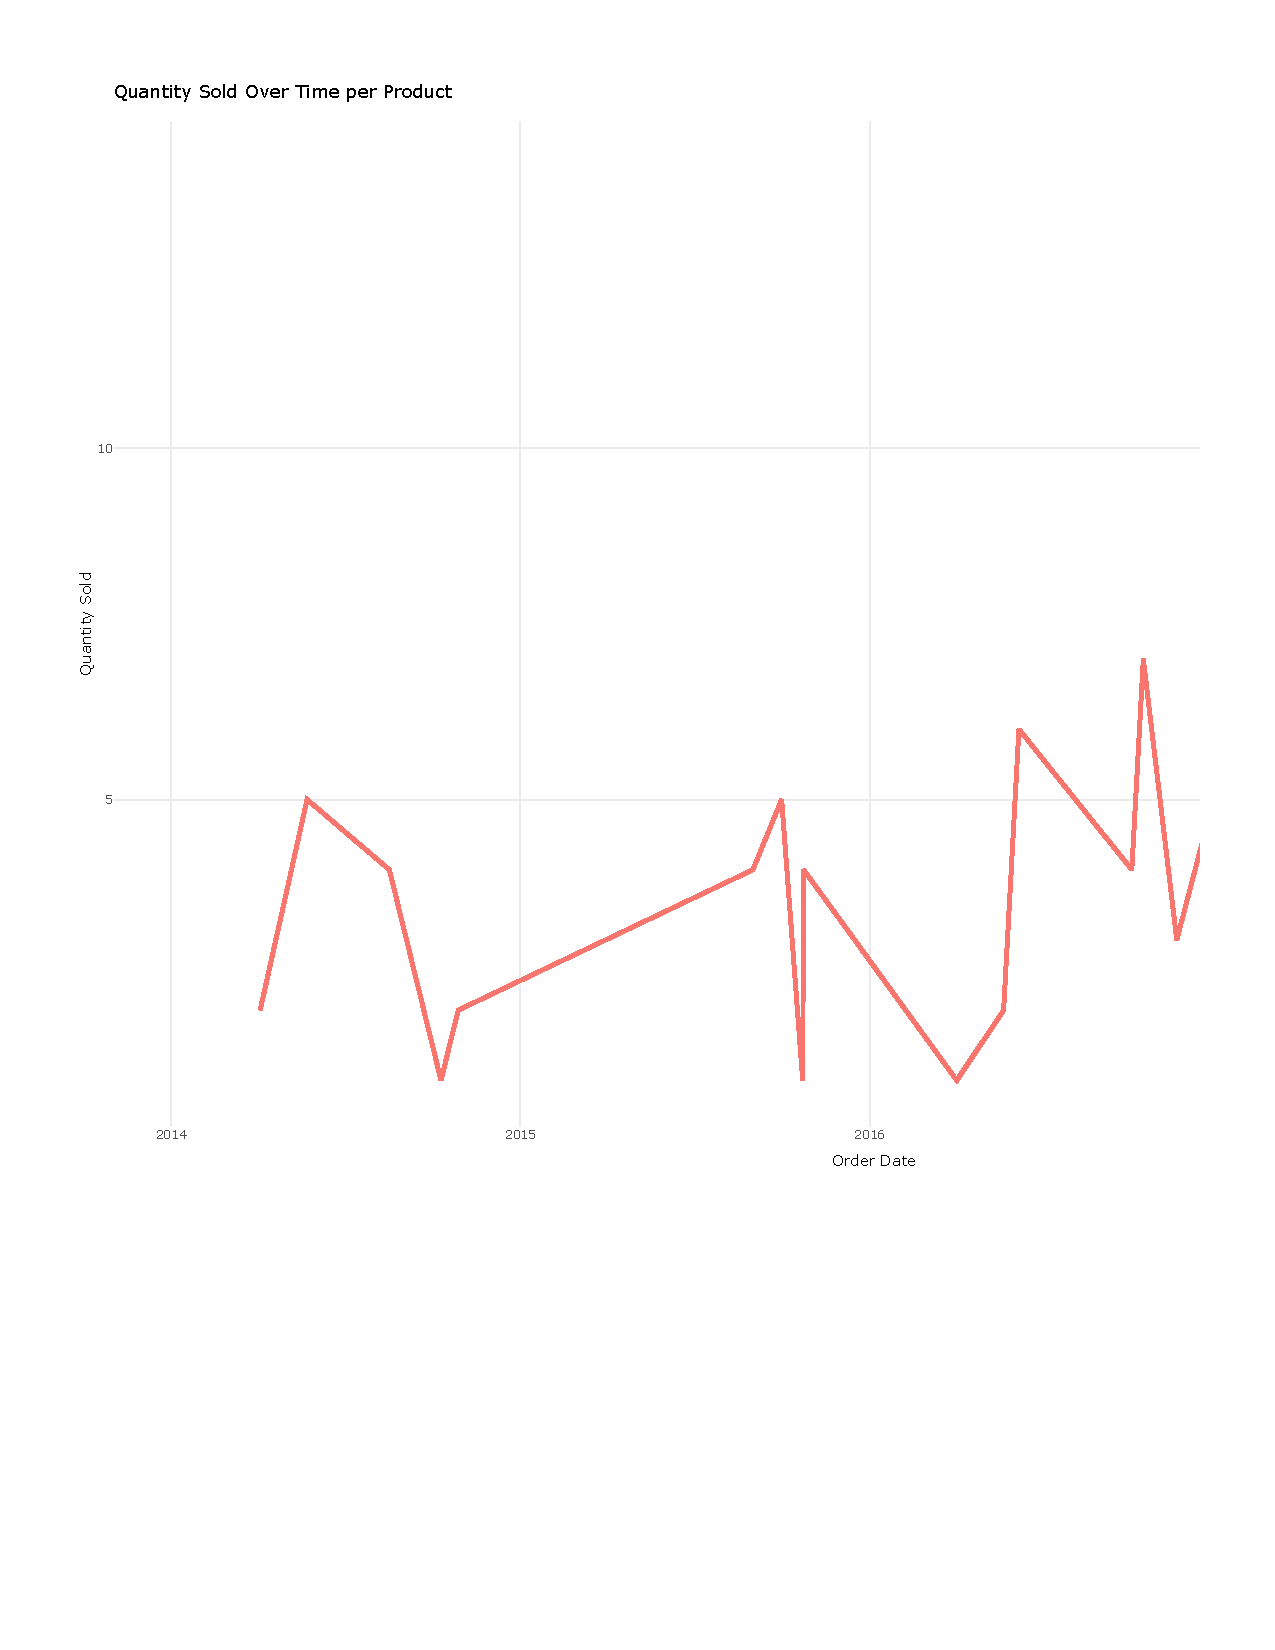
\includegraphics[keepaspectratio]{index_files/figure-pdf/Quantity_top_products-1.pdf}}

}

\caption{Figure x Sale quantity of the most popular products}

\end{figure}%

\textsubscript{Source:
\href{https://SJbrou.github.io/Supply_Chain_Data_Analysis/index.qmd.html}{Article
Notebook}}

Our proposed workaround is to aggregate products by their Sub\_Category,
and treating them as a single product for the rest of the assignment,
which we plotted in figure X.

\pandocbounded{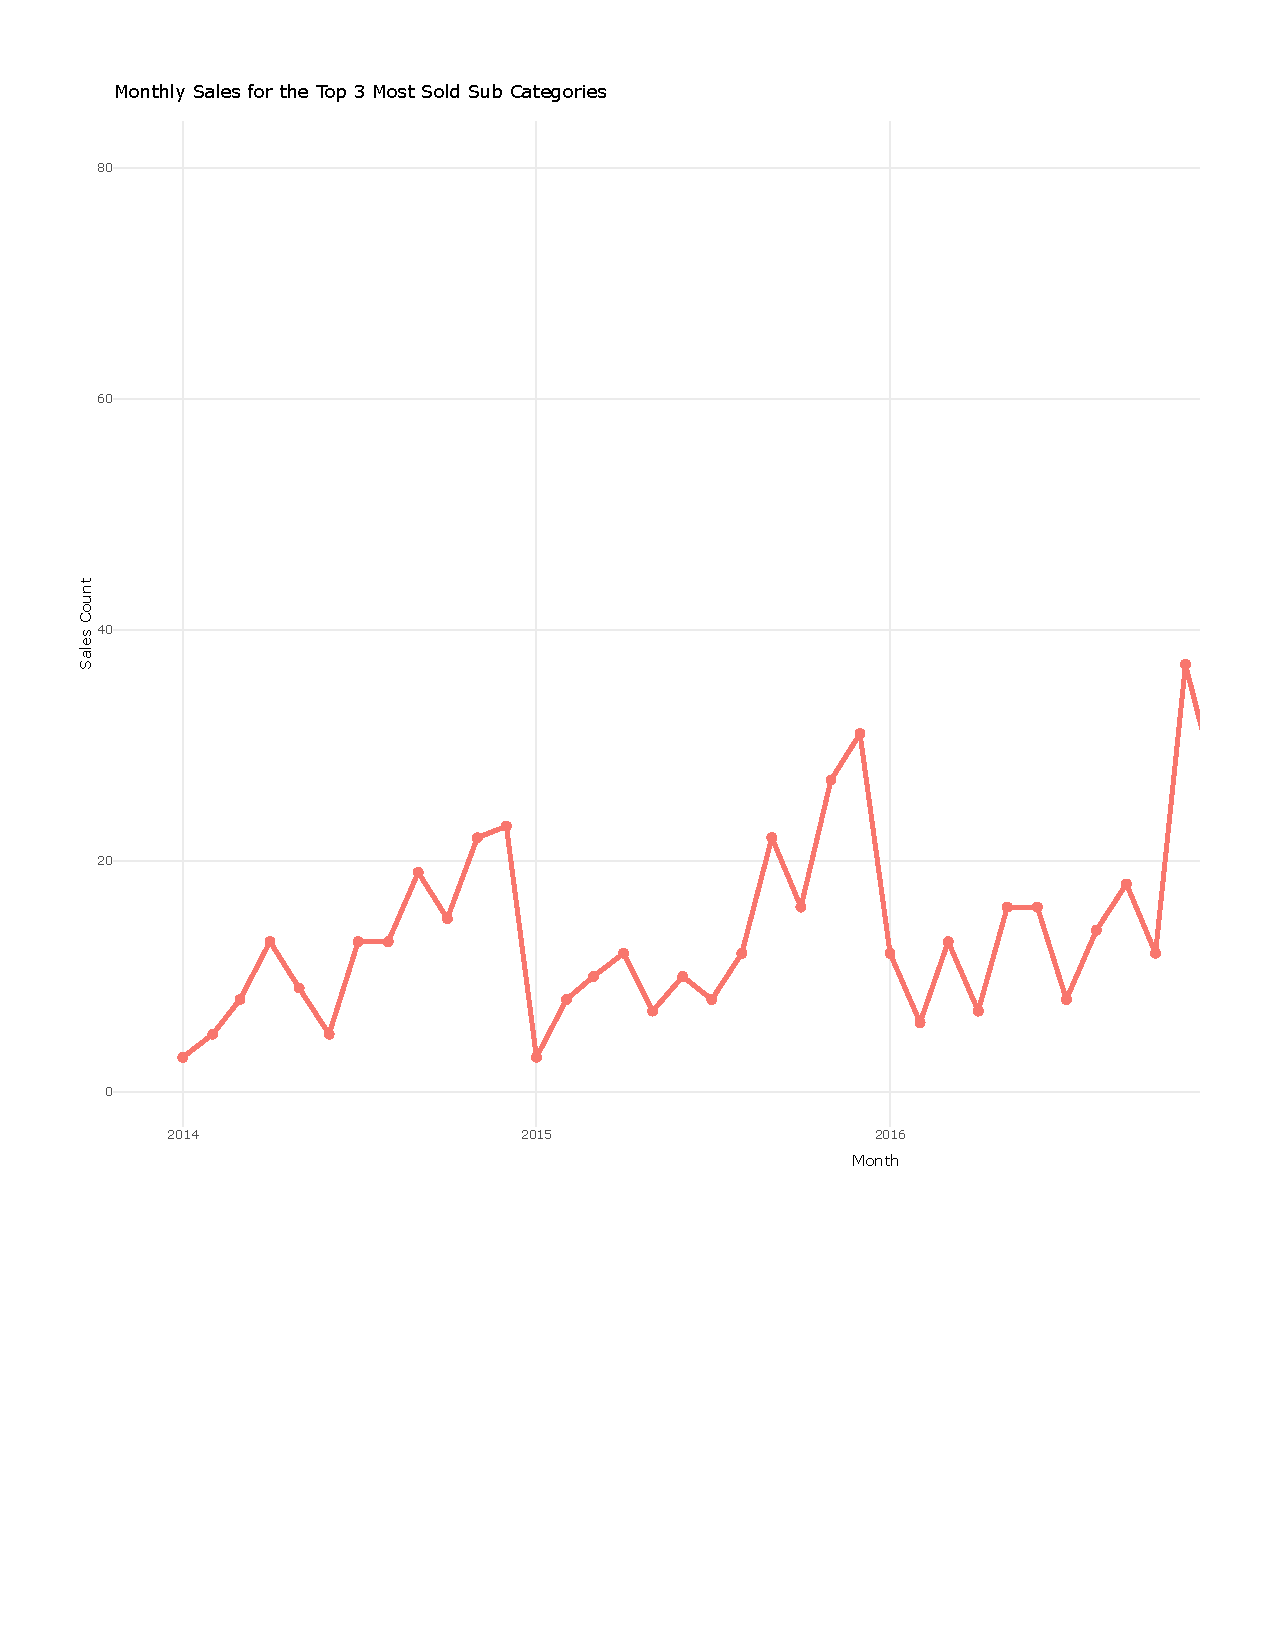
\includegraphics[keepaspectratio]{index_files/figure-pdf/Aggregated_Sub_Category_sales-1.pdf}}

\textsubscript{Source:
\href{https://SJbrou.github.io/Supply_Chain_Data_Analysis/index.qmd.html}{Article
Notebook}}

These aggregated sales start to show trends and seasonality, and are
much more useful to base predictions on! We will use these aggregated
sub-categories for the rest of the assignment.

To properly finish our data pre-processing we ran some statistics on the
aggregated sub-category sales. Table x contains soem descriptive
statistics.

\begin{longtable}[]{@{}lrrrrrr@{}}
\caption{Statistics for Sub\_Category quantity}\tabularnewline
\toprule\noalign{}
Sub\_Category & Min & Mean & Max & Sd & CI\_lower & CI\_upper \\
\midrule\noalign{}
\endfirsthead
\toprule\noalign{}
Sub\_Category & Min & Mean & Max & Sd & CI\_lower & CI\_upper \\
\midrule\noalign{}
\endhead
\bottomrule\noalign{}
\endlastfoot
Accessories & 1 & 3.84 & 14 & 2.28 & 3.68 & 4.00 \\
Appliances & 1 & 3.71 & 14 & 2.12 & 3.52 & 3.90 \\
Art & 1 & 3.77 & 14 & 2.13 & 3.62 & 3.92 \\
Binders & 1 & 3.92 & 14 & 2.29 & 3.80 & 4.04 \\
Bookcases & 1 & 3.81 & 13 & 2.28 & 3.51 & 4.11 \\
Chairs & 1 & 3.82 & 14 & 2.28 & 3.64 & 4.00 \\
Copiers & 1 & 3.44 & 9 & 1.83 & 3.01 & 3.87 \\
Envelopes & 1 & 3.57 & 9 & 2.05 & 3.32 & 3.82 \\
Fasteners & 1 & 4.21 & 14 & 2.41 & 3.89 & 4.53 \\
Furnishings & 1 & 3.72 & 14 & 2.16 & 3.58 & 3.86 \\
Labels & 1 & 3.85 & 14 & 2.35 & 3.61 & 4.09 \\
Machines & 1 & 3.83 & 11 & 2.17 & 3.43 & 4.23 \\
Paper & 1 & 3.78 & 14 & 2.23 & 3.66 & 3.90 \\
Phones & 1 & 3.70 & 14 & 2.19 & 3.56 & 3.84 \\
Storage & 1 & 3.73 & 14 & 2.19 & 3.58 & 3.88 \\
Supplies & 1 & 3.41 & 10 & 1.84 & 3.15 & 3.67 \\
Tables & 1 & 3.89 & 13 & 2.45 & 3.62 & 4.16 \\
\end{longtable}

\textsubscript{Source:
\href{https://SJbrou.github.io/Supply_Chain_Data_Analysis/index.qmd.html}{Article
Notebook}}

The statistics for the sales aggregated by product category look valid.
We can further inspect them by visualizing them as histogram and
visually check for anomalies. Figure y contains histograms of the
quantities per sub-category.

\pandocbounded{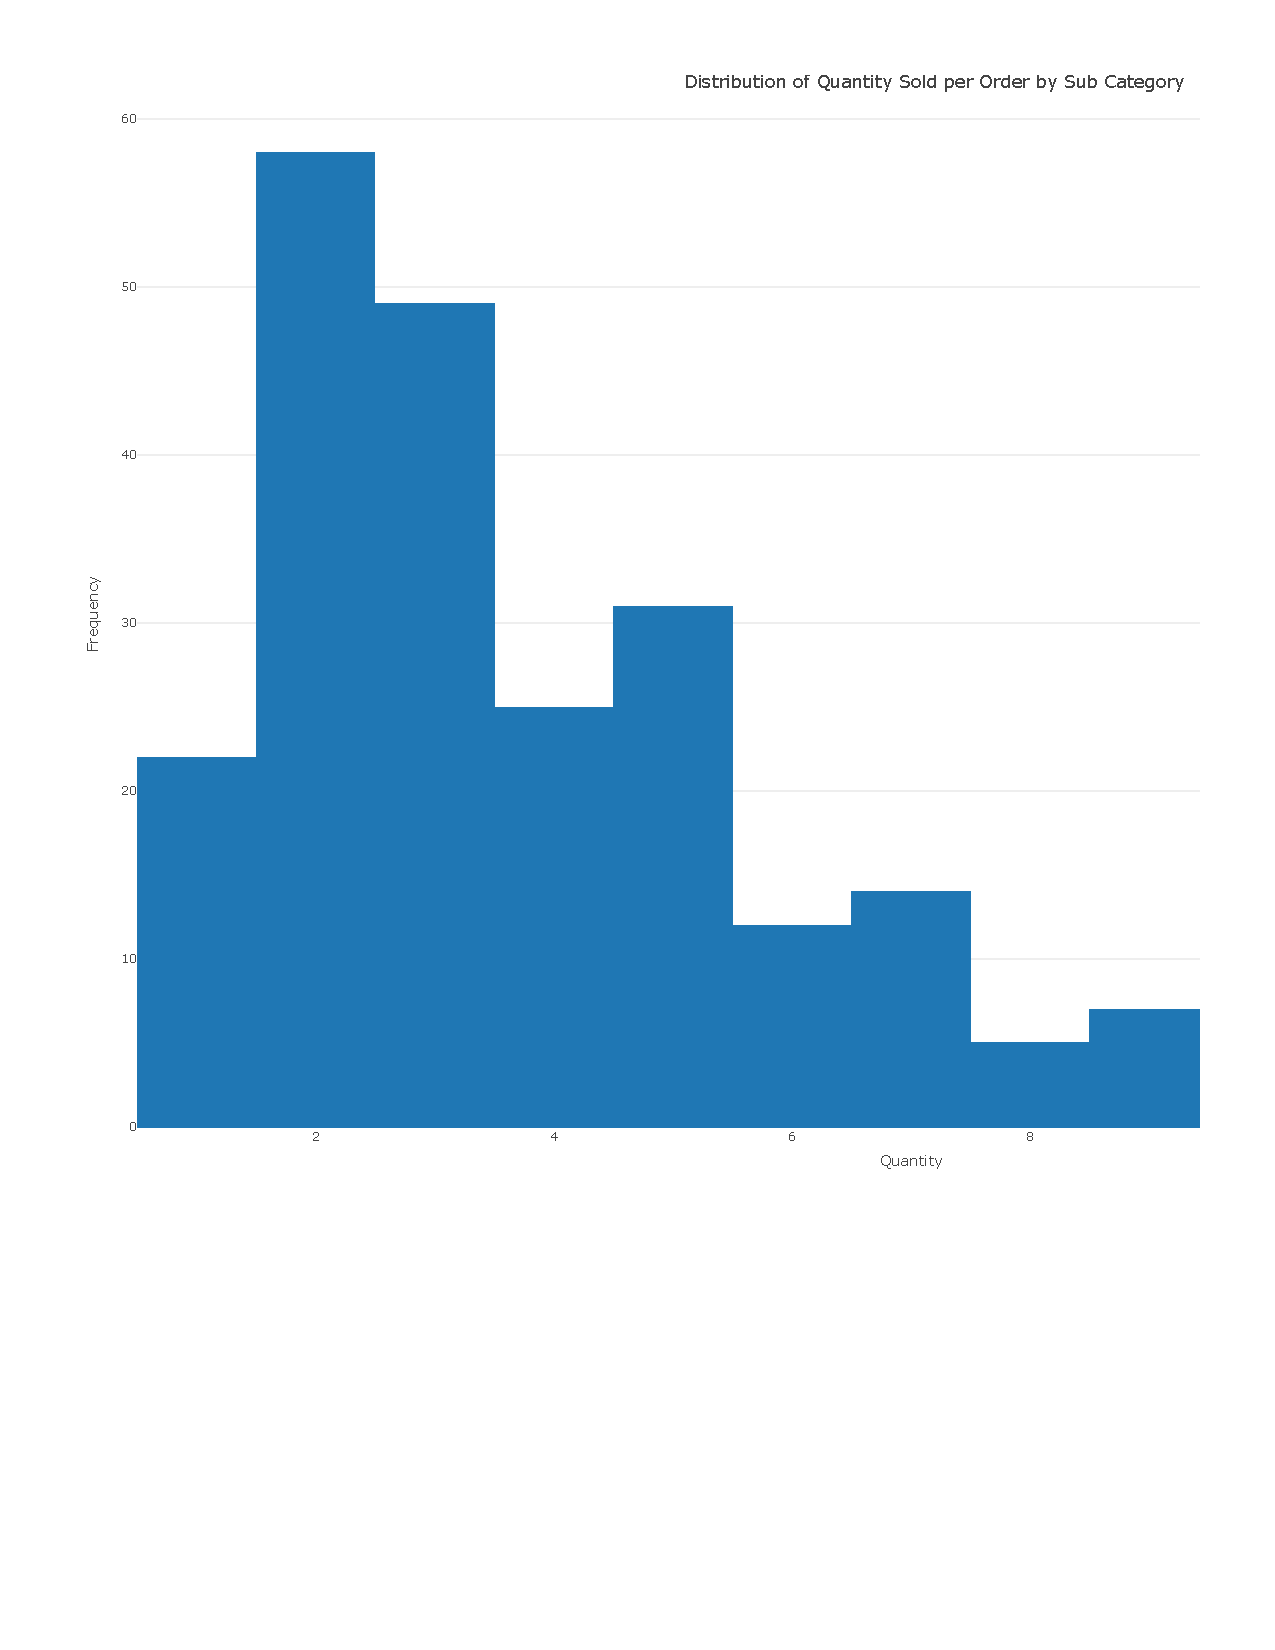
\includegraphics[keepaspectratio]{index_files/figure-pdf/sub_category_histograms-1.pdf}}

\textsubscript{Source:
\href{https://SJbrou.github.io/Supply_Chain_Data_Analysis/index.qmd.html}{Article
Notebook}}

The histograms show that the quantities are not normally distributed,
but have a right-skewed distribution. This is expected as most orders
contain a small number of items, but some orders contain a large number
of items. We will not remove these outliers as they are valid orders.

As the data we are going to use seems valid, we move on to exploring the
trends and visualizing our data.

\subsection{Data Visualization}\label{data-visualization}

some text for the visualization




\end{document}
